%%This is a very basic article template.
%%There is just one section and two subsections.
\documentclass[UTF8]{ctexart}
\title{第六章 JESD204B确定性时延}
\author{陈登}
\date{\today}

\bibliographystyle{plain}
\usepackage{graphicx}
\usepackage{float}
\usepackage{amsmath}
\usepackage{geometry}
\usepackage{fontspec}
\usepackage{algorithm}
\usepackage{algorithmicx}
\usepackage{algpseudocode}

\geometry{a4paper,centering,scale=0.9}
\usepackage[format=hang,font=small,textfont=it]{caption}
\usepackage[toc,page,title,titletoc,header]{appendix}
\usepackage[nottoc]{tocbibind}

\begin{document}

\section{JESD204B确定性时延}

JESD204B规定的两种需要实现确定性时延的Subclass,主要需要设计两部分的对齐策略。
一是帧层面的确定性时延,这一部分主要是保证在本地多帧时钟控制下,接收到的数据能同步的传输到接下来的模块中。
二是本地多帧时钟层面的确定性时延,这一部分主要保证各个设备间的本地多帧时钟能够同步,从而使整个系统之间能够有同样的收发节拍,能够将各个模块、设备之间的不确定性降到最低。

\subsubsection{相位同步问题}

在一些应用中,需要产生不同频率的多个信号,并且拥有相近的相位控制关系。
其中一种应用就是医疗设备中的扫描设备,医疗成像中使用了许多个不同频率的信号。
当信号穿过身体,他们的相位产生了扭曲,并且这些相位中的扭曲能够用来生成图像。
如果一个信号芯片能够生成所有需要的频率,它也能够更简单的获得受控制的相位对齐。
但是如果一个应用需要更多的时钟输出(多余一个芯片能够提供的),他就需要通过级联的方法得到足够的输出。

\begin{figure}[H]
\centering
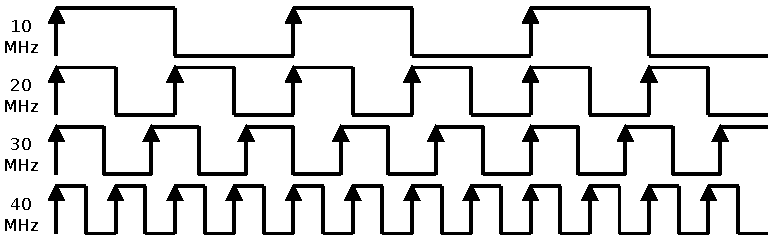
\includegraphics[width=18cm]{./img/signal_phase_sync.pdf}
\caption{信号相位同步}
\label{fig:signal_phase_sync}
\end{figure}

图\ref{fig:signal_phase_sync}显示的一组10、20、30和40MHz的信号在相位上同步。
所有的信号频率都是 0MHz的倍数,并且他们在最低频率的边沿上对齐。
如果10MHz信号并不包含在内,则应该能够发现20、30和40MHz的信号能够被想象中的10MHz信号对齐。
图\ref{fig:understanding_lcm_gcd_frequencies}显示在这个实例中,12.288Mhz 和 30.72MHz 信号在相位上同步。
在这个例子中,一个构想出来的6.144MHz信号能够同12.288MHz和30.72MHz信号拥有同样的上升沿。
6.144MHz即为12.288MHz和30.72MHz的最大公约数。
另一个值得关注的频率是一个最小的频率,能够符合其他所有信号的上升沿。
在这个例子中是61.44MHz,即为12.288MHz和30.72MHz的最小公倍数。

\begin{figure}[H]
\centering
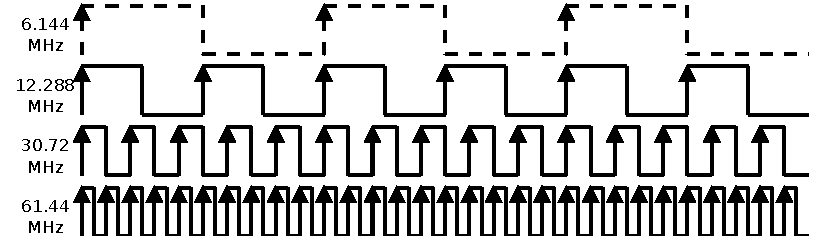
\includegraphics[width=18cm]{./img/understanding_lcm_gcd_frequencies.pdf}
\caption{理解频率的最大公约数和最小公倍数}
\label{fig:understanding_lcm_gcd_frequencies}
\end{figure}

\subsubsection{相位分歧问题}

由于不均衡的路径长度或者使用了没有分频的芯片,引起的时延通常是确定的。一旦分频参与进来,就会产生随机的相位关系。当一个频率被D分频,将会产生D种可能的相位状态。考虑图\ref{fig:ambiguous_phase_produced_by_division}所示的信号被4分频的情况。

\begin{figure}[H]
\centering
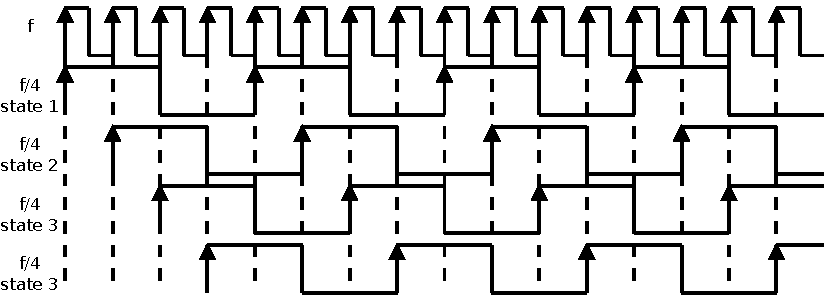
\includegraphics[width=18cm]{./img/ambiguous_phase_produced_by_division.pdf}
\caption{由分频引起的相位分歧}
\label{fig:ambiguous_phase_produced_by_division}
\end{figure}

在这个例子中有4种可能的状态,所有的相位都和初始信号同步,但是各个状态之间却并不同步。如果不采取恰当措施的话,当多个芯片通过同一个时钟,来产生相同的分频信号时,产生的信号之间就会发生相位同步问题。

\subsection{帧层面的确定性时延实现}

link之间的确定性时延定义在收端和发端的以帧为基础的并行数据层面,即保证在帧时钟域。
不同link间的时延保证需要以帧时钟周期为单位,并且能够通过寄存器配置完成具体时延的设置。
这样的设置需要在上电或者link重连阶段能够有一定的重复性。

为了达成确定性时延,需要满足以下两个条件:

\begin{itemize}
\item 对于发端设备,所有lane之间的ILA序列产生必须同时进行,这也同时保证了数据流同时产生。
\item 对于收端设备,每个lane收到的数据必须在各个物理通道间设置缓存。收端缓冲需要在一个预先定义好的时刻,同时释放所有lane的数据。这个特殊时刻指的是可编程数量帧周期接收缓冲时延\footnote{Rx Buffer Delay}(在本地多帧时钟边界后)。
\end{itemize}

ILAS生成和接收端缓冲释放对齐,都是以接收端和发送端的本地多帧时钟为标准。
所以,确定性时延的最小不确定性依赖于接收端和发送端之间本地多帧时钟的对齐程度。

为了实现确定性时延的协议要求,系统设计时需要保证以下几点:

\begin{itemize}
\item 多帧长度必须大于link间可能存在的最大时延。
\item $RDB * T_f$的值必须大于link间可能存在的最大时延。
\item $RDB$的值,依照帧周期,必须介于1到K之间。
\end{itemize}

以上三条的目的是保证RBD够大,能够使接收端缓冲在释放前,所有lane的发送端数据被收到。
最终JESD204B link间的时延为$RDB * T_f$。
JESD204B link间的确定性时延要求接收端设备能够缓冲收到所有lane的ILA序列或者用户数据,在接收端缓冲能被释放前。
缓冲必须在本地多帧时钟边界过后,RBD个帧周期之后释放。
为了能够释放缓冲,需要满足所有lane都有“有效数据”存在各自的接收端缓冲中,这里有“效数据”指:

\begin{itemize}
\item 如果ILA序列发送到了接收端缓冲中,那么有效数据指的是ILA序列的开端。
\item 如果ILA序列没有发送到接收端缓冲中,那么有效数据指的就是完整ILA序列之后出现的样本数据。在这种情况下接收端缓冲将会比第一种情况迟4个多帧释放。
\end{itemize}

link间的时延可由下式表示,这也是所谓的确定性时延需要保证的确定部分:

$$Delay_{LINK} = \delta T_{LMFC} = TX \quad delay + Lane \quad Delay + RX \quad delay$$

其中,$TX \quad delay$指的是从发送端ILA序列产生,并出现在发送端SerDes的输出端口上的时间;$Lane \quad delay$指的是穿过外部物理信道的时延;$RX \quad delay$指的是从接收端SerDes输入到通入缓冲输出的时延。ILA序列的开端或者用户数的开端,将会在本地多帧时钟边加上RBD个帧时钟周期时出现在缓冲输出;$\delta T_{LMFC}$指的是link间的全部时延,指的是发送端本地多帧时钟上升沿到接收端本地多帧时钟加上$T_f * RBD$上升沿之间的时延。

接收端缓冲的最小大小取决于最早可能到达接收端缓冲输入的数据和下一个接收端缓冲释放条件产生之间的时差。

Subclass 0类设备并不支持确定性时延。

\subsection{本地多帧时钟层面的确定性时延}

由帧层面的确定性时延处理方法可以总结出来,各个设备之间的同步最关键在于同步各自的本地多帧时钟边界,即需要各个设备能够将自己的本地多帧时钟对准到所需要的边界上。
Subclass 1类和Subclass 2类设备最大的区别就在于本地多帧时钟的对齐方式上,Subclass 1类设备需要额外的外部时钟信号SYSREF来保证同步,而Subclass 2类设备则需要通过自身的SYNC~信号来保证同步。

在保证本地多帧时钟同步之后,之后对于帧同步的处理都是相同的。

\subsubsection{Subclass 1类设备的本地多帧时钟同步}

对于Subclass 1设备来说,发端和收端设备的对齐本地多帧时钟信号是通过SYSREF信号完成,所以SYSREF信号必须分部到所有的转换器和逻辑设备上。
系统中延时的不确定性通过高精度的SYSREF和设备时钟信号对进行最小化。
并且建议由同一个设备产生发送和接收设备的SYSREF信号。

介于存在各种SYSREF信号类型(periodic、one-shot、gapped periodic),各种时钟信号生成设备也许不支持所有的协议要求的SYSREF信号选项,所以建议系统在一般操作时能够主动的关闭SYSREF信号。

对于Subclass 1类设备,需要满足以下要求:

\begin{itemize}
\item 发送逻辑设备需要能够处理生成SYSREF信号的请求,接收设备能够使能时钟生成模块,能够对系统中所有设备产生一个或多个SYSREF脉冲。如果使能了,生成SYSREF信号的请求能够在link在SYNC~接口上产生重同步请求时处理。
\item 发送逻辑设备需要能够处理生成SYSREF信号的请求,发送设备能够使能时钟生成模块,能够对系统中所有设备产生一个或多个SYSREF脉冲。如果使能了,生成SYSREF信号的请求能够在link在SYNC~接口上产生重同步请求时处理。
\item 发送和接收设备需要有能力决定是否校正本地帧和多帧时钟到SYSREF脉冲。实现这一功能的细节由设计者决定,但是有以下三种种可能的选项供选择。
	\begin{itemize}
	\item 每一个SYSREF脉冲需要被设备验证,以决定现有的本地多帧时钟相位和帧时钟是否需要对齐。
	\item 一个设备可以通过设备的输入引脚或者控制接口命令来决定是否用下一个收到的SYSREF脉冲强制对齐本地多帧时钟和本地帧时钟相位。
	\item 一个设备可以通过设备的输入引脚或者控制接口命令来决定是否忽略所有的SYSREF脉冲。
	\end{itemize}
\end{itemize}

需要指出的是,对于Subclass 1设备,本地多帧时钟和帧时钟的重对齐是基于SYSREF信号的,并且只有在设备初始化或者link出现失败需要重同步的情况下才进行。
在处理SYSREF时序问题上,发送和接收设备需要能够设置本地设备时钟数量,讲采样到的SYSREF信号延迟相应数量的本地设备时钟,再将本地多帧时钟对齐到延时后的上升沿上。

对于应用来说,确定性时延需要等于一个完整的多帧周期,将接收缓冲时延的值设置成K。
这样强制将接收缓存的释放十几规定在一个多帧边界上。

当接收设备所有的lane完成码群同步后,将在之后的任意一个本地多帧时钟上升沿改变SYNC~信号输出通知发送端。
很短的一段时间后,发送收到了SYNC~信号的变化,在之后的第一个本地多帧时钟上升沿开始传输ILAS。
之后收端讲开始检测所有lane的ILAS开端,并将输入压入每一个lane的缓冲。
在下一个本地多帧时钟上升沿,收端设备将会在所有lane上检测到有效的ILA数据,并且释放所有的缓冲。
JESD204B link间收端设备输出的数据将会有一个多帧周期的固定时延。

对于应用设备,有不同的确定性时延要求,接收缓冲时延的值需要设置成小于K的值。

总而言之,针对Subclass 1类设备,参考信号SYSREF使收端和发端设备能获得同步的本地多帧时钟。
具体的实现,是设备在收到SYSREF信号后,收端和发端对该信号延时一定数量的设备时钟,这个数量应该是能够配置的,目的消除不同信号之间的相位差异,达到同步。
最后收发端都使用延时后的信号校正本地多帧时钟信号,保证时延正确。

同步了本地多帧时钟后,针对可能存在的不同设备间的时延,采取了收端通过接受缓冲缓存已接受数据并在固定时机释放的机制保证不同lane、link之间的确定性时延。
接收缓冲时延是一个可编程的延时数量,用以保证在固定数量octet时钟周期后同时释放缓存。

总结以上描述,Subclass 1类设备的本地多帧时钟同步主要是通过对齐外部的SYSREF信号。
需要处理的是两个问题,一个是SYSREF信号到达各个设备的同步问题,一个是设备自己的本地多帧时钟与SYSREF信号对齐的时机问题。

\paragraph{SYSREF信号同步}

针对第一个问题,协议要求所有设备的本地多帧时钟必须要相同,但是SYSREF也是一个时钟信号,在传输和产生过程中,也会产生一定的时延,比如布线布局上存在的时延差问题。
所以在Subclass 1类设备中通过自己的设备时钟,当SYSREF信号到达后,产生指定数量的功能性时延后再对本地多帧时钟进行对齐,以保证各个设备的本地多帧时钟是同步的。
而对于时延数量的设置需要根据具体的电路设计来确定。

\paragraph{本地多帧时钟与SYSREF对齐时机}

针对第二个问题,协议并没有强制设定具体的对齐时机,但给出了一些建议。
发送端和接收端设备需要有能力决定是否校正本地帧和多帧时钟到SYSREF脉冲。
这一功能实现的细节由设计者决定,但是提供了三种可能的选项供选择。

\subsubsection{Subclass 2设备的本地多帧时钟同步}

Subclass 2设备的时延也依靠正确的对齐发送和接收设备的本地多帧时钟,但是不能依赖于附加的SYSREF信号。
之前对于SYSREF信号之外的描述都基本适用于Subclass 2类设备,尤其是对本地多帧时钟的使用。
由于需要取代对SYSREF信号的对齐依赖,系统的发送端需要加强对SYNC~信号的精确捕捉
由于已知的发送端和接收端多帧周期的相位区别,正确的对齐必须选择通过发送转换器对齐接收逻辑设备,还是通过接收转换器对齐发送逻辑设备。

Subclass 2类设备的确定性时延精确度基于SYNC~信号变化的传输和捕获精度。
在link的发送和接收终端,设备在产生和捕获SYNC~信号的过程中会产生一定数量的延时。
对于这些时延的控制程度将会限制Subclass 2类设备的确定性时延的实现。
由设备时钟产生或者捕获的SYNC~信号相较于由内部时钟对齐或者检测到的时钟产生或者捕获的SYNC~信号受到的PVT影响更小。
想要最小化时延的不确定性,取决于SYNC~信号产生和捕获过程中的PVT影响,并且在link两端都需要考虑这一问题。
延时的变化范围主要还是取决于制造商的工艺水平。
要达到传输的最大速率,就是将时序边界的PVT边界视作0。

Subclass 2设备不同于Subclass 1设备,Subclass 2设备的本地多帧时钟对齐要更加的复杂。
Subclass 2设备由于没有共同的外部时钟源,所以本地多帧时钟的同步完全依赖于SYNC~接口的信号变化,并且对于接收端和发送端的处理有主从的区别。
总的来说,Subclass 2类设备的本地多帧时钟同步主要分为模数转换器和逻辑设备的同步,数模转换器与逻辑设备的同步两种情况考虑。
为了能够使本地多帧时钟同步在收发两端都有一个具体的参考指标,还需要建立一套对于SYNC~信号的采样处理机制。

\paragraph{由接收设备生成的SYNC~信号}

由接收设备产生的SYNC~信号经常生成于内部帧时钟并且将取消SYNC~请求的边界对齐到接收设备的LMFC边界。
取消SYNC~请求的边界信号往往携带了接收设备的本地多帧时钟相位信息。
通常情况下,帧时钟会直接被用来驱动SYNC~发送到发送设备。
当设备的时钟频率允许时,SYNC~信号在发送前需要重对齐到设备时钟。

\paragraph{调整分辨率和调整时钟}

在转换设备中,本地多帧时钟相位能够在调整分辨率的增量范围内被调整。
调整分辨率被定义为本地多帧时钟能够被调整的最小时间间隔。
它使用link中最高频率的设备时钟来驱动,这样就好于转换器的设备时钟来驱动的。
可以采用以下几条来定义调整时钟:

\begin{itemize}
\item 调整时钟周期等同于link的调整分辨率,并且调整范围能够通过控制接口编辑。
\item 转换器的本地帧时钟和本地多帧时钟需要对齐到调整时钟的上升沿。
\item 调整时钟的相位对齐到设备时钟的相位,为的是保证时序。
\end{itemize}

如果调整分辨率要求的比转换器设备时钟周期和帧时钟周期都要高,那么就需要为转换器开发一个高速的调整时钟,从它的设备时钟调整到link所需要的调整分辨率。
以下有两种可能情况:

\begin{itemize}
\item 当转换设备时钟快于逻辑设备时钟时,调整分辨率即为转换器时钟的周期。
\item 当转换设备时钟慢于逻辑设备时钟时,调整分辨率即为逻辑设备时钟的周期。\footnote{注意:只有当调整分辨率的要求高于转换器时钟周期时,转换器的本地多帧时钟边界不需要对齐到设备时钟。}
\end{itemize}

\paragraph{发送设备检测分辨率}

在发送X设备中,SYNC~取消请求的信号是由SYNC~解码器检测到的。
SYNC~取消请求信号携带了接收设备的本地多帧时钟相位信息。
SYNC~取消请求信号的检测是基于一个检测时钟,他的周期等同于本link的检测分辨率。
这个时钟的周期可能不会大于发送设备本地帧时钟的周期,与此同时在SYNC~信号检测中也要考虑错误报告的问题。
这个子类设备延时的精确度依赖于检测分辨率要高于或等于调整分辨率。
这里有一种可能,发送逻辑设备的检测分辨率可能不同于link的调整分辨率。
为了能够从一个慢速设备时钟中获得更好的检测分辨率,可能需要在发送设备中开发一个更高速的检测时钟。

\paragraph{SYNC~取消请求信号检测和检测间隔}

正如接收和发送设备时钟可能不会一直相位对齐到一个link的一个帧时钟上,SYNC~取消请求信号必须使用发送本地帧时钟去检测来增加错误报告的检测精度。
存在这样一种可能,link的调整分辨率会比检测分辨率粗糙。
根据这种情况,在一次调整过程中可能存在多个检测点。
如果在这种情况下,检测分辨率步骤中的一个间隔能够被很好的定义去适配调整分辨率。
检测间隔现在能够允许发送设备在检测中基于转换器的能力去调整。
一个检测间隔有一下特性:

\begin{itemize}
\item 检测间隔只存在于当link的调整分辨率比检测分辨率更加粗糙的情况下。
\item 检测间隔被设置成等同于系统地调整分辨率。
\end{itemize}

\paragraph{建立本地多帧时钟同步方法}

模数转换器和逻辑设备的同步:

在模数转换器与逻辑设备同步的前提下,是由模数转换器的本地多帧时钟对齐到逻辑设备的本地多帧时钟。
由于模数转换器是作为发端设备,需要始终监视来自逻辑设备的SYNC~信号。
SYNC~信号当中其实承载了收端逻辑设备的本地多帧时钟信息,发端收到这一信息后就要能够判断出是否出现相位差。
并且决定是否将本地多帧时钟同这一边沿对齐。

这一操作的精度主要取决于模数转换器的调整分辨率。
如果模数转换器的调整分辨率要优于帧时钟周期,模数转换器将会把本地多帧时钟和帧时钟在SYNC~信号到来是都进行重置。
如果模数转换器的调整分辨率并不优于帧时钟周期,它的调整时钟将会与帧时钟对齐,并且不会对帧时钟进行重置。

在时钟进行重新调整的过程中需要花费一定的时间,这个具体的时间是由制造商决定的,并且在这段时间内持续的发送/K28.5/。

数模转换器与逻辑设备的同步:

发送端设备作为主设备,接收端设备作为从设备,目标就是通过发送端设备收到的SYNC~变化边界通过对比发送端设备本地的本地多帧时钟边界判断是否需要调整。
由于之前协议的规定,接收端改变SYNC~信号的时机是来自接收端的本地多帧时钟,这就意味着发送端得到SYNC~变化实质上是接收端的本地多帧时钟边界。
当发送端收到这个信号后就会将这个信号对自己的本地多帧时钟进行比较,从而判断是否符合同步条件,是否需要调整。
当发送端设备准确判断出需要调整时,会在接下来传输的ILA序列中添加调整参数,这几个参数是ADJCNT(调整步数)、ADJDIR(调整方向)、PHADJ(调整使能)。
这种情况下发送端不会发送具体数据,纯粹是利用ILA序列进行本地多帧时钟的同步对齐。
而接收端设备在收到ILA序列中对于调整的需求时就将对自己的本地多帧时钟进行调整,完成调整后在新的本地多帧时钟上升沿在SYNC~接口发送一个错误报告。
发送端口又会根据这个错误报告的本地多帧时钟边界判断是否需要继续调整,是否在合适的范围内。
如此循环直到同步建立,当T发送端认为同步成功后就会发送具体的数据,并置低PHADJ。

具体发送端的检测有限状态机如图\ref{fig:TX_logic_device_subclass_2_control_machine}所示。

\begin{figure}[H]
\centering
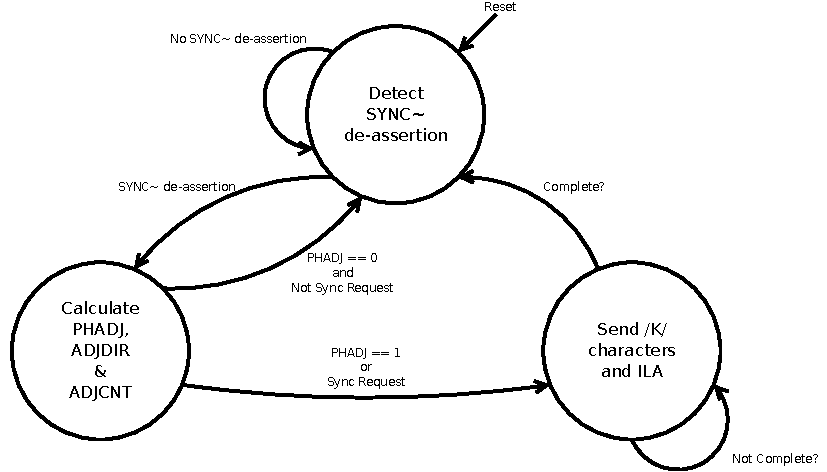
\includegraphics[width=12cm]{./img/TX_logic_device_subclass_2_control_machine.pdf}
\caption{Subclass 2类设备发送端的检测有限状态机}
\label{fig:TX_logic_device_subclass_2_control_machine}
\end{figure}

具体接收端的调整有限状态机如图\ref{fig:Subclass_2_DAC_adjustment_machine}所示。

\begin{figure}[H]
\centering
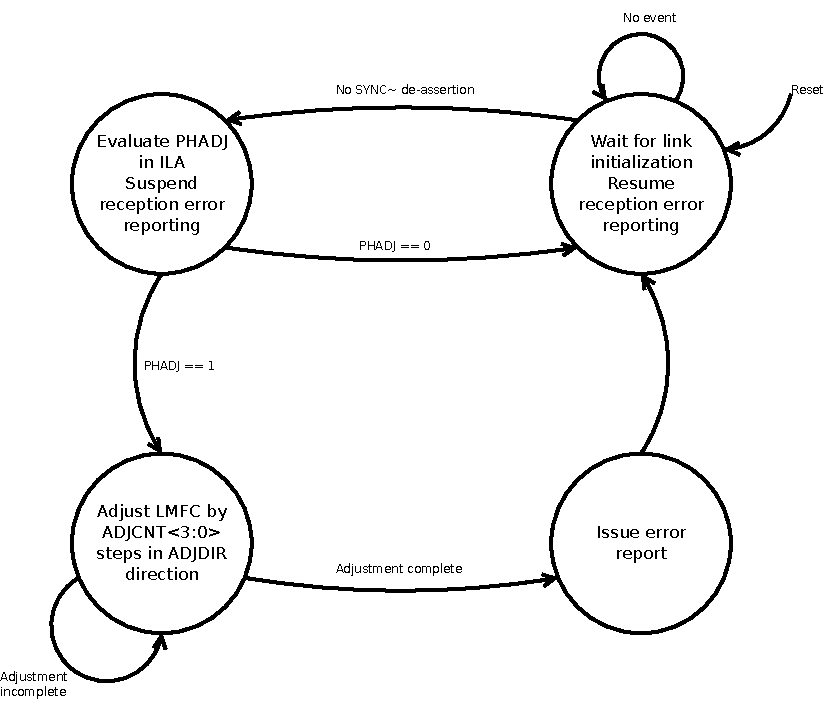
\includegraphics[width=12cm]{./img/Subclass_2_DAC_adjustment_machine.pdf}
\caption{Subclass 2类设备接收端的调整有限状态机}
\label{fig:Subclass_2_DAC_adjustment_machine}
\end{figure}

具体的调整流程如图\ref{fig:deter_latency_subclass_2}所示。

\begin{figure}[H]
\centering
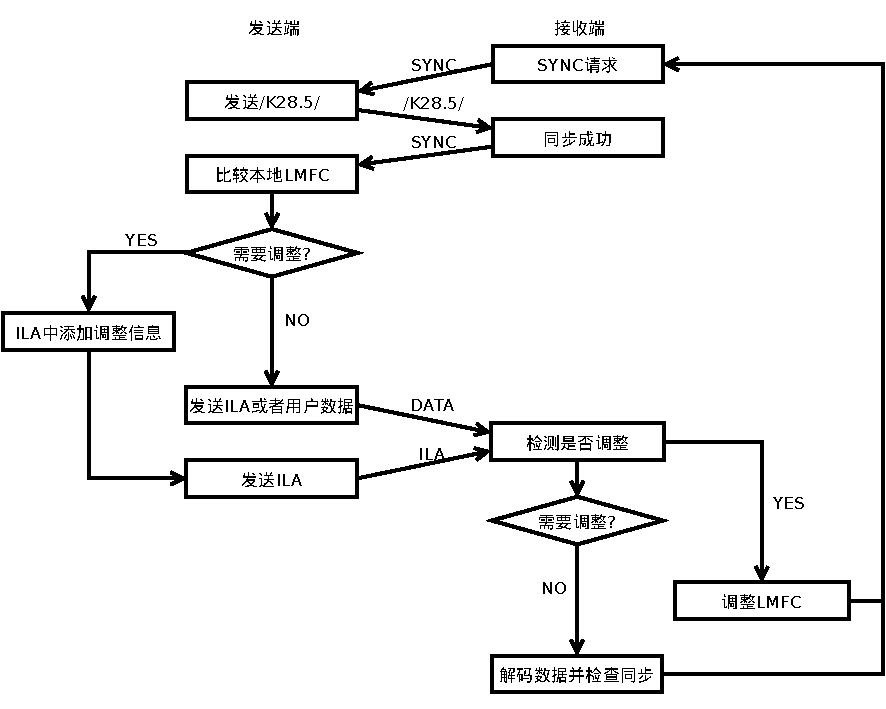
\includegraphics[width=18cm]{./img/deter_latency_subclass_2.pdf}
\caption{Subclass 2类设备本地多帧时钟同步过程}
\label{fig:deter_latency_subclass_2}
\end{figure}

一位的PHADJ被定义为有调整请求。
ADJCNT<3:0>被定义为调整分辨率的步骤计数。
ADJDIR被定义为调整的方向。
ADJDIR如果为1表示延时,如果为0表示超前。
当数模转换器发现PHADJ在处理ILAS过程中被置高,它将会相应调整请求,调整它的本地多帧时钟。
根据ADJCNT的数量调整调整分辨率步骤的数量,根据ADJDIR决定调整方向。
当完成调整后,数模转换器会产生一个错误报告到发送逻辑设备,并将新的本地多帧时钟相位信息作为一个调整请求的共识。
使用PHADJ、ADJCNT和ADJDIR可以使能迭代的调整数模转换器的本地多帧时钟直到它的相位能够对齐到发送逻辑设备的本地多帧时钟。

在检测SYNC~取消请求同步信号的状态下,发送逻辑设备根据自己的检测时钟持续的检测信号。
当一个测SYNC~取消请求同步信号被检测到后,发送逻辑设备会判断是否需要调整接收端的本地多帧时钟到自己的本地多帧时钟。
如果基于检测分辨率或者检测间隔的发送端本地多帧时钟边界和检测到的SYNC~信号存在差异,就需要进行调整。
如果发送端判断不需要调整,并且测SYNC~取消请求同步信号并没有作为来自数模转换器的同步请求信号,那么就不需要进行调整请求,并且发送逻辑设备重新进入到SYNC~采样状态。
如果发送端判断需要调整,或者测SYNC~取消请求同步信号作为来自数模转换器的同步请求信号,那么一个link的初始化操作将会被执行。
如果调整是必须的,将会通过置高PHADJ来发送一个请求,并配置ADJCNT<3:0>作为调整大小,ADJDIR作为调整方向。

如果发送端判断不需要调整,并且测SYNC~取消请求同步信号并没有作为来自数模转换器的同步请求信号,PHADJ将会被置低。
在参数被设置后,发送逻辑设备会发送一连串/K28.5/字符的数据流和一个ILAS,在这之中有三个调整参数被嵌入。
配置数据的校验和将被重新计算。
一旦ILA被发送,则发送端将会回到持续对SYNC~信号的采样阶段。
数模转换器将会通过一个错误报告知会相位的改变并包含新的数模转换器的本地多帧时钟相位信息。
这个报告可以循环迭代用来反复调整本地多帧时钟使其保持同步。

数模转换器会相应来自逻辑设备的请求。
在重置之后,调整模块会监视接口,观察是否有link初始化条件。
在这个状态下会接收到多个/K/字符,并在其后跟随ILAS。
在ILAS中会检测PHADJ、ADJDIR和ADJCNT。
如果PHADJ没有被置高,就不需要调整,数模转换器将会处理之后的数据。
状态机将会继续监视接口可能的下一个link初始化条件。
如果PHADJ被置高,那么状态机将会对数模转换器的帧时钟相位和本地多帧时钟相位做一个时序的调整。
调整的方向和大小由ADJDIR和ADJCNT决定。
发送逻辑设备能够精确的计算ADJCNT,数模转换器制造商必须能够定义数模转换器调整分辨率用数模转换器设备时钟周期数。

如果ADJCNT等于0,那么一个零调整将被执行。
一旦本地多帧时钟调整完成,数模转换器会通过SYNC~接口触发一个错误报告到发送逻辑设备。
一旦错误报告被发送,那么状态机将重新回到检测下一个link初始化的时间中。

这样的调整机制是建立在两个基础上。

\begin{itemize}
\item 一是发送端能够精确的比较SYNC~变化和本地多帧时钟的差异,于是需要在发送端建立了检测分辨率和检测间隙机制。实际上就是对本地设备时钟的精度有一定的要求,能够准确判断本地多帧时钟和SYNC~信号变化之间的相位差的差距具体时延数。而本地多帧时钟对齐的精确度也是由这一机制来保证,设备时钟的精确度直接决定了检测的精度。
\item 二是接收端能够根据收到的调整数据对本地相位进行调整,于是在接收端建立了调整分辨率和调整时钟机制,调整时钟直接决定了调整的范围和精度。
\end{itemize}

\bibliography{../../bib/serdes}
\end{document}
